\documentclass[10pt,t]{beamer}

\usepackage[utf8]{inputenc}
\usepackage[T1]{fontenc}
\usepackage{graphicx}
\usepackage{grffile}
\usepackage{longtable}
\usepackage{wrapfig}
\usepackage{rotating}
\usepackage[normalem]{ulem}
\usepackage{amsmath}
\usepackage{textcomp}
\usepackage{amssymb}
\usepackage{capt-of}
\usepackage{hyperref}

\input beamer_setup

\usetheme{default}
% ---------------------------------------------------------------------
% ---------------------------------------------------------------------
\begin{document}

\title[]{Applications of Single Footprint Retrievals : \newline Humidity above DCCs and Trace Gases}
% \author{Sergio DeSouza-Machado, Larrabee Strow} \institute{Department of Physics, JCET\\
% University of Maryland Baltimore County (UMBC)
% {Jing Feng, Yi Huang} \institute{Department of Atmospheric and Ocean Sciences, \\McGill University, Canada}}
\author{Sergio DeSouza-Machado$^{a}$, Larrabee Strow$^{a}$ \newline Jing Feng$^{b}$, Yi Huang$^{b}$}
\institute{$^{a}$Department of Physics, JCET, University of Maryland Baltimore County (UMBC) \newline
  $^{b}$Department of Atmospheric and Ocean Sciences, McGill University, Canada}
\date{October 4, 2018}
% ---------------------------------------------------------------------
% ---------------------------------------------------------------------
\begin{frame}
  \titlepage
\end{frame}
% ---------------------------------------------------------------------
% ---------------------------------------------------------------------
\begin{frame}
  \frametitle{Overview}

  \begin{itemize}
  \item Reminding you about our Single Footprint Retrievals
    \begin{itemize}
    \item Surf temp, \textcolor{red}{100 layer}
      T(z),\water(z),O3(z),\textcolor{red}{ice and water clouds}    
    \item \textcolor{red}{100 layer retrieval takes $\le$ 2 seconds per
        single FOV}    
    \item 8-12 hours per granule, 240 processors do entire day in 12 hours
    \item 100 layers (could be sped up if we use trapezoids?)
    \item Matlab based loops (will be sped up with f77/f90)
    \end{itemize}
  \item Used to test SARTA performance
  \item Allows radiosonde inter-comparisons under some cloud cover
  \item Examine single footprint fitting residuals to uncover issues
  \item "Validations"
    \begin{itemize}
    \item AIRS L2 ice ODs and MODIS water cloud ODs
    \item GRUAN sondes
    \end{itemize}
  \item Show and tell
    \begin{itemize}
    \item Hurricane Florence
    \item Looking at humidity above DCC
    \item CO retrievals (post-processing after thermodynamic retrieval)
    \end{itemize}
  \end{itemize}
\end{frame}
% ---------------------------------------------------------------------
% ---------------------------------------------------------------------
\section{Retrievals}
% ---------------------------------------------------------------------
% ---------------------------------------------------------------------
\begin{frame}
  \frametitle{Single Footprint Retrievals}
  \begin{itemize}
  \item My QA depends on closeness to start profile (T/WV/O3 stemp)
    and bias(900 \wn, 1231 \wn) : low QA is not bad news
  \item Cloud Representation : NWP multilayer cloud converted to Two Slab
    Clouds (ice/water)
  \item OEM methodology, so DOF is a natural diagnostic
  \item smoothing by combination of Tikonov matrices,
    $\sigma(i)^2 e^{-((i-j)/h)^2}$, climatology
  \end{itemize}

  \begin{columns}[T] % align columns
    \begin{column}{.38\textwidth}

      \small

      Single Footprint Retrievals, DeSouza-Machado {\em et. al., Atmos. Meas. Tech.}, 2018 \newline
      % https://doi.org/10.5194/amt-11-529-2018

      Evaluation of Radiative Transfer Models with Clouds, Aumann {\em et. al., J. Geophys. Res},2018
      % \newline 10.1029/2017JD028063

    \end{column}%
    \hfill%
    \begin{column}{.58\textwidth}

      \centering
      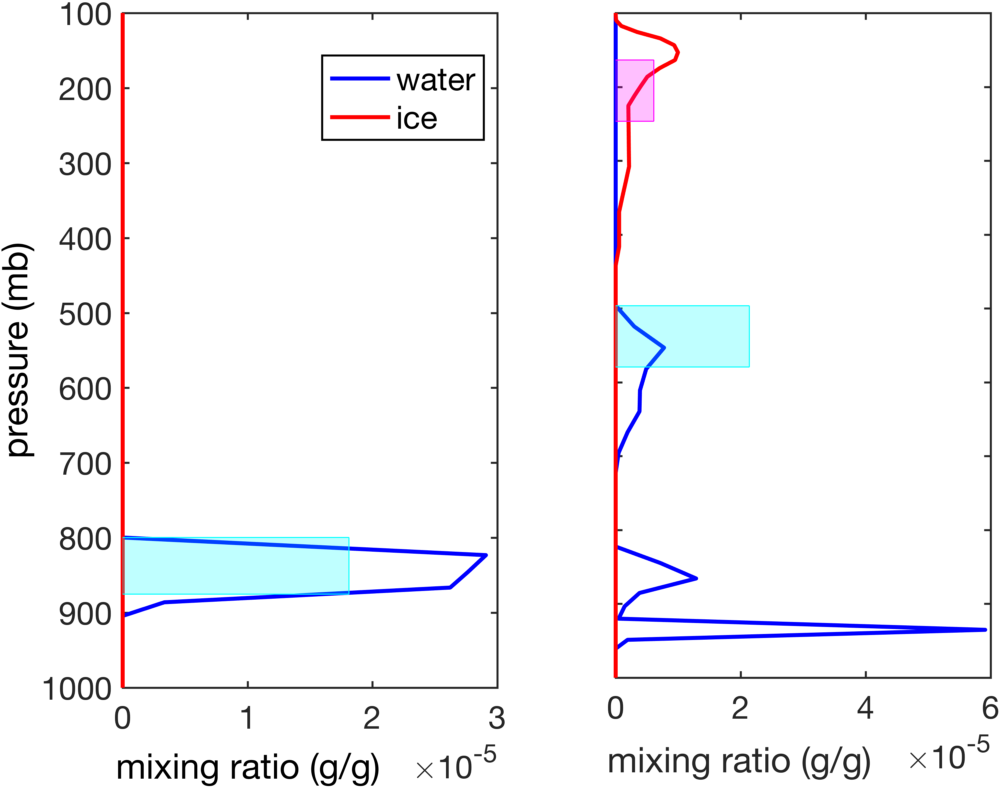
\includegraphics[width=0.75\linewidth]{Figs/FigsRetr/clouds_profileG040_271_321_lls.png}
    \end{column}%
  \end{columns}

\end{frame}
% ---------------------------------------------------------------------
% ---------------------------------------------------------------------
\section{Ice/Water clouds}
% ---------------------------------------------------------------------
% ---------------------------------------------------------------------
\begin{frame}
  \frametitle{Ice Cloud ODs 2011/03/11 day}

  \hspace{0.50in} AIRS L2 \hspace{1.75in} UMBC \\
  \begin{center}
    \dlandgraph{0.48}{Figs/FigsRetr/JPL_Feb2018_CompareMagicSonde/kahn_iceOD_day_2011_03_11_log.pdf}{Figs/FigsRetr/JPL_Feb2018_CompareMagicSonde/umbc_iceOD_day_2011_03_11_log.pdf}
  \end{center}

  Have looked at cldforcing, and the differences in cloud OD (UMBC vs L2)
  are typically in regions of "low" forcing, need to investigate further

\end{frame}
% ---------------------------------------------------------------------
\begin{frame}
  \frametitle{Water Cloud ODs 2011/03/11 day}
  % \emph{note the colorbar for MODIS L3 spans a wider range}\\
  (different sensor/wavelengths used in retrieval, so expect different
  magnitude ODs ... but patterns are similar)

  \hspace{0.50in} MODIS L3 \hspace{1.75in} UMBC \\
  \begin{center}
    \dlandgraph{0.48}{Figs/FigsRetr/JPL_Feb2018_CompareMagicSonde/modisL3_waterOD_day_2011_03_11_log.pdf}{Figs/FigsRetr/JPL_Feb2018_CompareMagicSonde/umbc_waterOD_day_2011_03_11_log.pdf}
  \end{center}
\end{frame}
% ---------------------------------------------------------------------
\begin{frame}
  \frametitle{2011/03/11 g039 : DCC over TWP}
  \noindent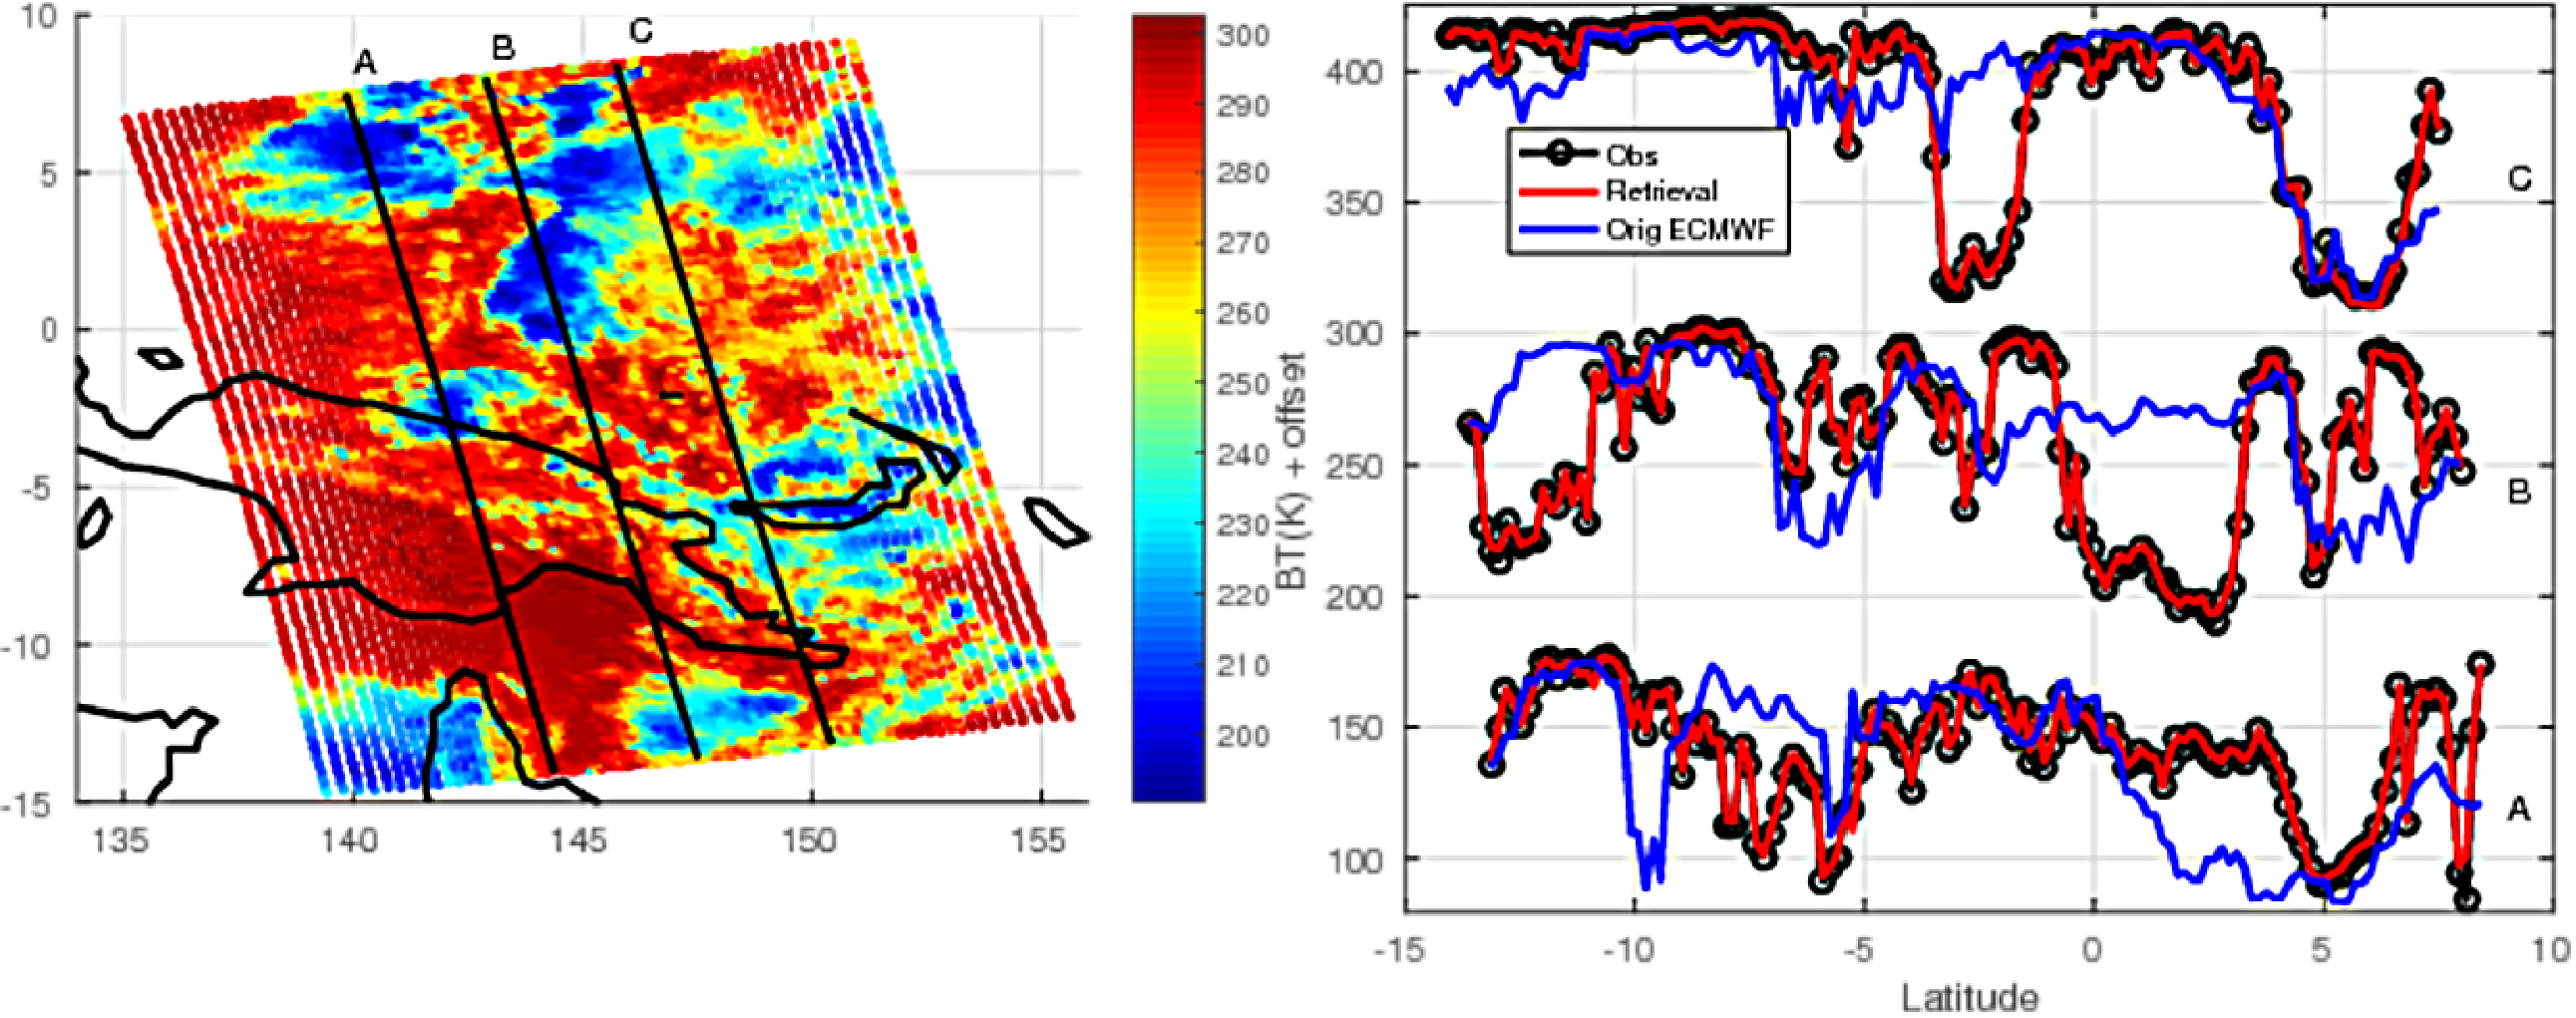
\includegraphics[width=\textwidth]{Figs/FigsRetr/AIRS_STM_Apr17/gran039_2011_03_11_bt1231_scatter_obs_3lines.pdf}

  BT 1231 \wn observations and calculations, in Kelvin.\newline

  \vspace{-0.2in} Left panel : AIRS observations for Granule 039 on March
  11, 2011. The lines are at three different AIRS scan angles. \newline

  \vspace{-0.2in} Right panel : BT1231 Observations (black) compared to
  calculations using the original ECMWF model fields (blue) and with the
  mitigated/retrieved cloud fields (red).
  
\end{frame}
% ---------------------------------------------------------------------
\begin{frame}
  \frametitle{Ice CldTop Heights}

  \hspace{0.25in} ECMWF \hspace{1.00in} UMBC retr \hspace{1.0in} MODIS L2  \\
  \begin{center}
    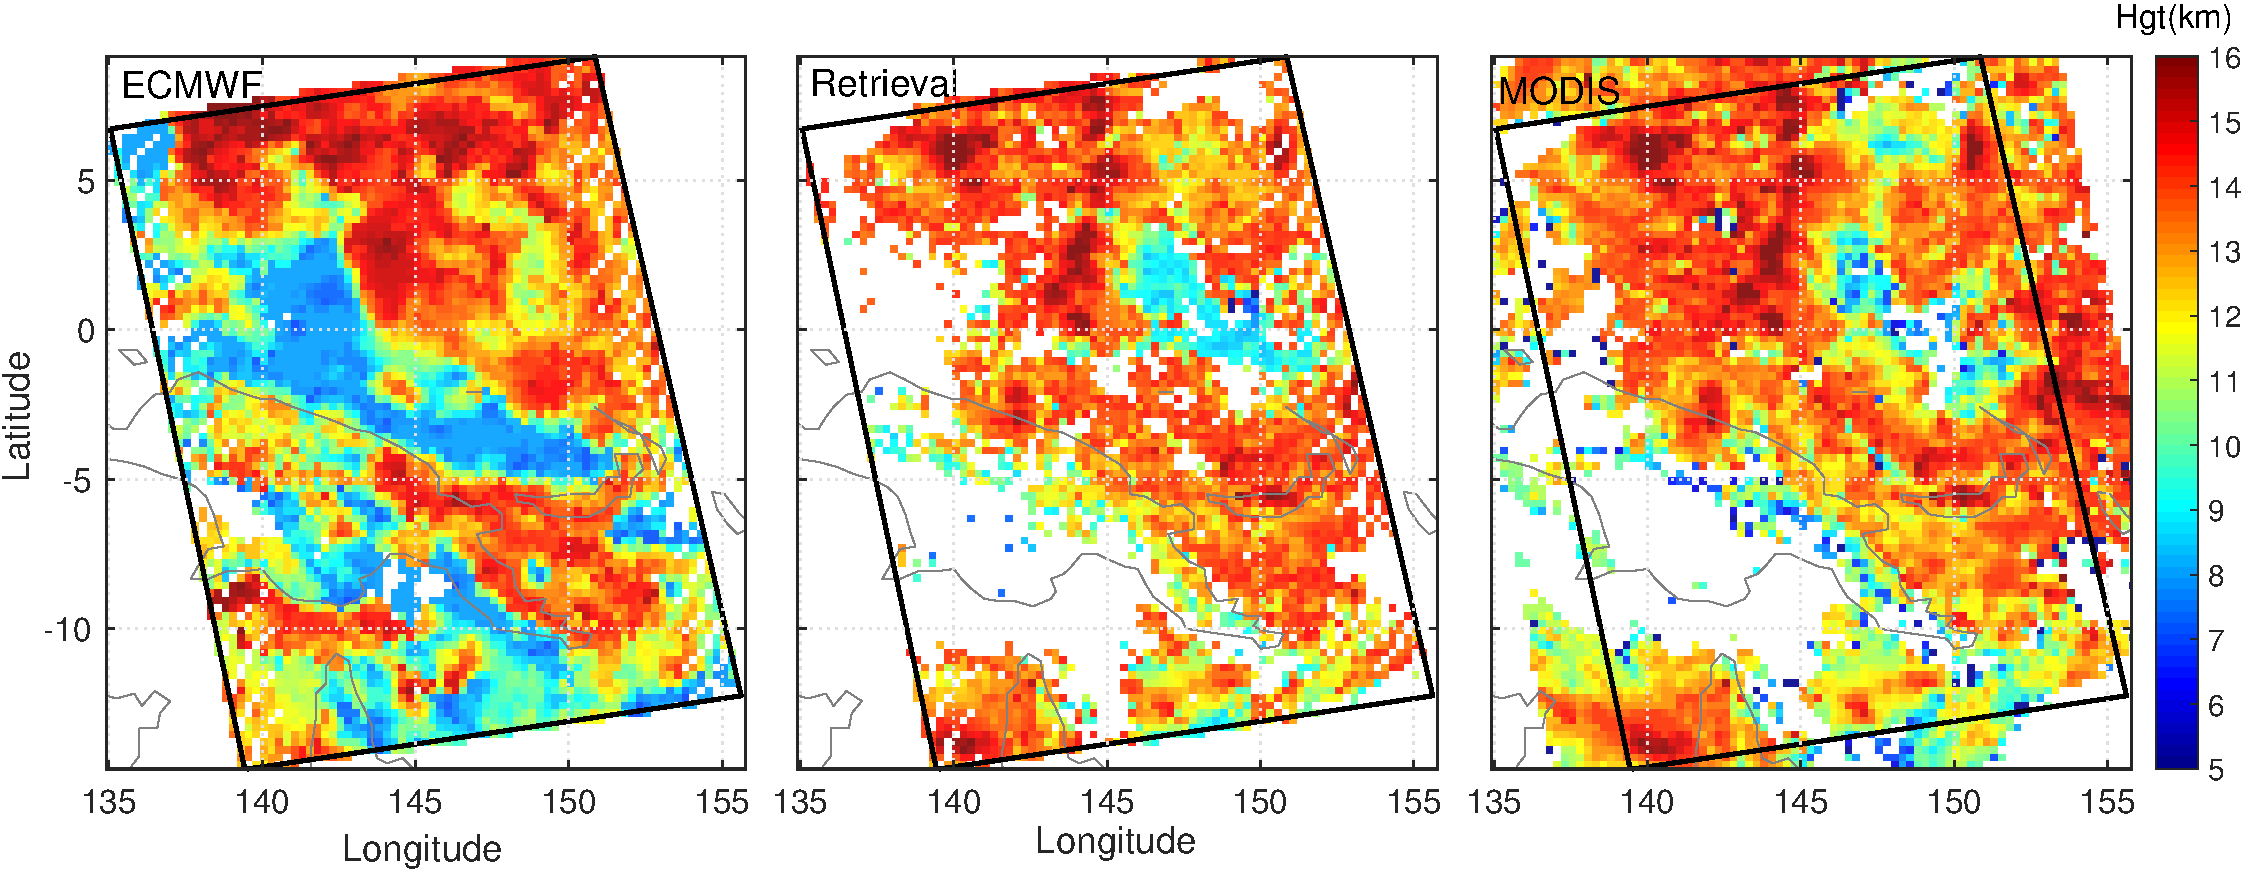
\includegraphics[width=0.95\linewidth]{Figs/FigsRetr/cldheight_v2.pdf}
  \end{center}

  Ice clouds with OD $\le$ 0.5 have been removed from plots \\
  Note similarity to BT1231 obs (high clouds = cold obs)
  
\end{frame}
% ---------------------------------------------------------------------
\begin{frame}
  \frametitle{DOFS and ice OD comparisons}

  \hspace{0.50in} DOFS \hspace{1.75in} Ice OD  \\
  \begin{center}
    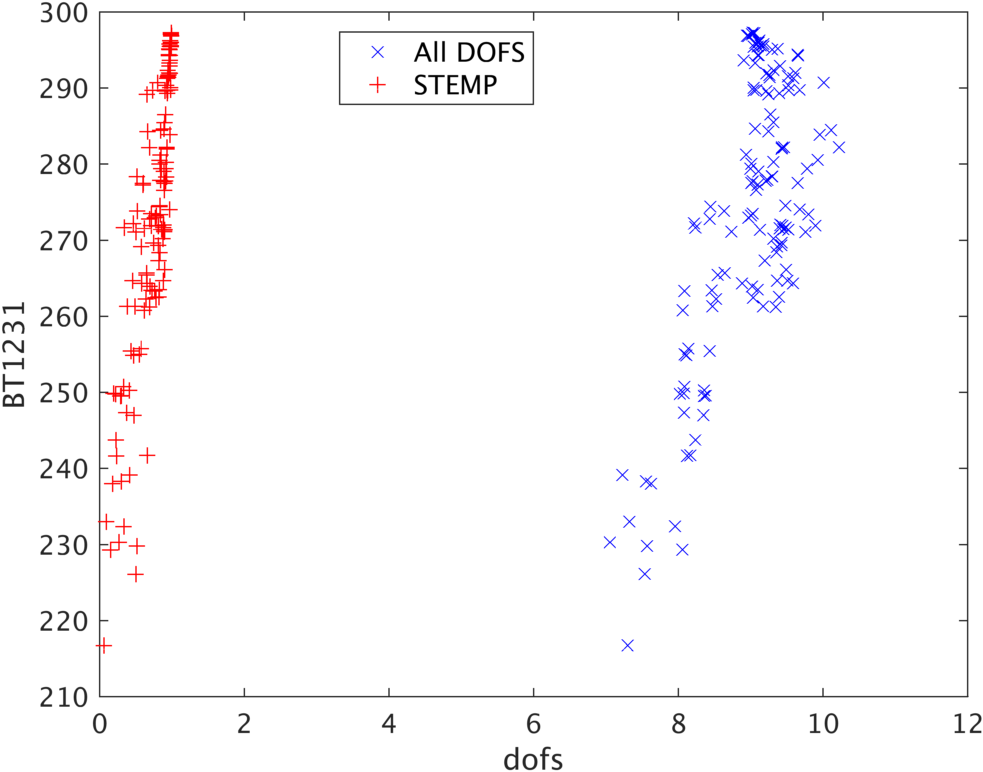
\includegraphics[width=0.45\linewidth]{Figs/FigsRetr/AIRS_STM_Apr17/dofs_all_stemp_2011_03_11.png}
    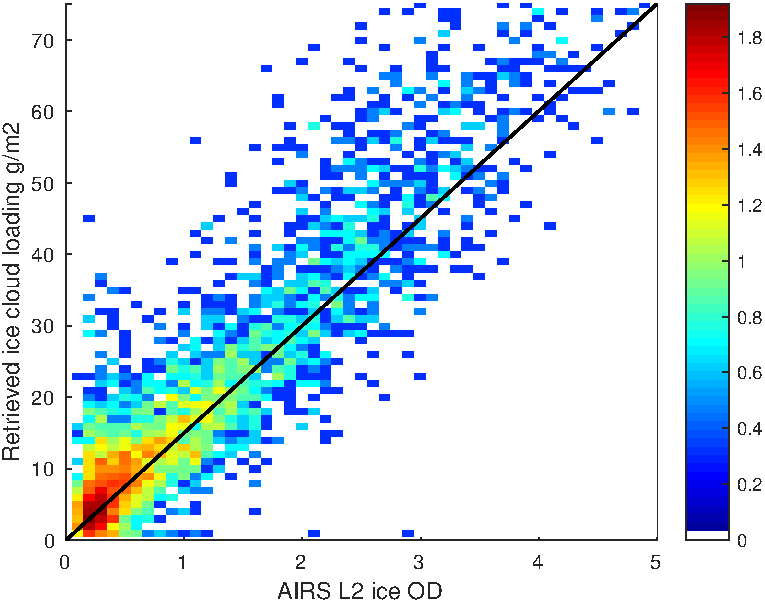
\includegraphics[width=0.45\linewidth]{Figs/FigsRetr/AIRS_STM_Apr17/cloud1_OD_G039_new_may23_2016.pdf}
  \end{center}

  DOF scale with obs BT 1231 : \textcolor{red}{Red crosses for stemp
    (between 0 and 1)}, \textcolor{blue}{blue crosses : all DOF (between 6
    and 14)}

  Ice OD : UMBC cloud loading vs AIRS L2 : colorbar is log10(number of
  points)

\end{frame}
% ---------------------------------------------------------------------
% ---------------------------------------------------------------------
\section{Sondes}
% ---------------------------------------------------------------------
% ---------------------------------------------------------------------
\begin{frame}
  \frametitle{Lindenberg, Germany GRUAN sondes \newline 52.21N, 14.12 E, 98
    m asl}

  \begin{itemize}
  \item 3200 sonde launches over a few years, ($\sim$ 220 each month)
  \item Select AIRS ovepasses within $\pm$ 1 hour and 100 km of sonde
    launch, gives 80-100 "nearest" AIRS obs per sonde
  \item Match AIRS observations to ERA thermodynamic/cloud profiles (252455
    "nearest" AIRS obs)
  \item Compare retrievals to sonde, sonde*AK and ERA
  \item Look at results as function of DOF
  \end{itemize}

  \vspace{0.125in} Wide variety of atmospheric conditions
  \begin{itemize}
  \item Surf temp varies from from 275 K (winter) to 295 K (summer); col
    water from 8 to 26 mm
  \item Clouds varied from none to DCC : Mean cloud forcing each month
    (Surftemp-BT1231 obs) = 15 K
  \end{itemize}
\end{frame}
% ---------------------------------------------------------------------
\begin{frame}
  \frametitle{Sonde-UMBC Retrieval}
  Divide the retrievals in quantiles of DOF, look at 4 quantile ranges\\

  \begin{small}
    \begin{table}[h]
      \begin{center}
        \begin{tabular}{lcccc}
          \hline
          Cloud     & Quantile & DOF range & CldEffect(K) &  Number \\
          condition & range    &           & (rough)      & AIRS obs \\
          \hline
          Very Thick cloud & 0.0-0.1 & 0.00-3.12 & > 50  & 2769 \\
          Thick cloud      & 0.1-0.5 & 3.12-4.29 & 20-50 & 43699 \\
          Medium Cloud     & 0.5-0.9 & 4.29-6.84 & 2-20  & 84579 \\
          Thin/no cloud    & 0.9-1.0 & 6.38-8.65 & < 2 & 24742 \\
          \hline
        \end{tabular}
      \end{center}
    \end{table}
  \end{small}

  \begin{center}
    \noindent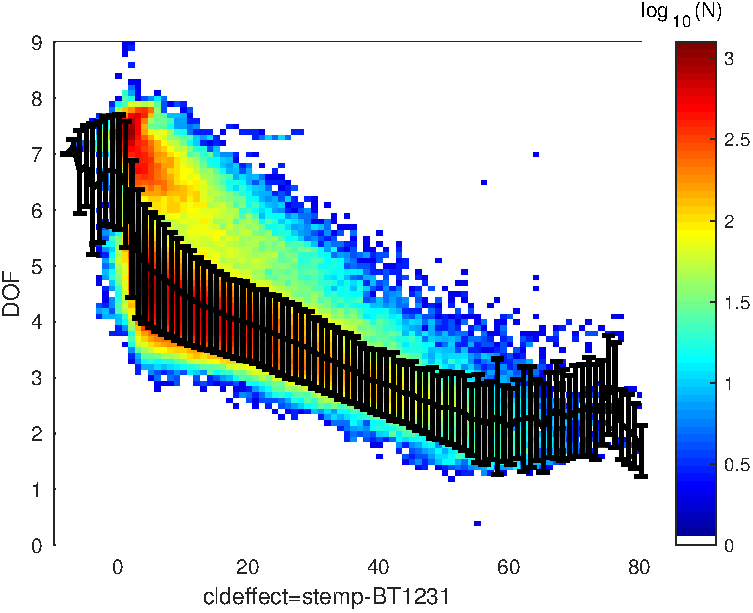
\includegraphics[width=0.45\textwidth]{Figs/FigsRetr/AIRS_STM_Apr18/dofs_vs_cldeffect_iSondeList_5_iStemp_ColWV_4_xvers_5_iSubset_1_dofALL.pdf}
  \end{center}
\end{frame}

% 0-0.1 (thick cloud), 0.1-0.5 (medium/thick clouds) 0.5-0.9 (thin cloud) 0.9-1.0 (almost clear)\\
% 0-3.12 (2769), 3.12-4.29 (43699),4.29-6.84(84579),6.38-8.65(24742)
% ---------------------------------------------------------------------
\begin{frame}
  \frametitle{Sonde-UMBC Retrieval}
  Divide the retrievals in quantiles of DOF, look at 4 quantile ranges\\
  \textcolor{red}{As expected biggest problems when clouds are thickest
    (low DOF)}; otherwise <sonde-retrieval> is typically within 1 K, 20\%
  RH

  \vspace{0.1in}
  T(z)  \hspace{3.0in} RH(z) \\
  \begin{center}
    \dlandgraph{0.48}{Figs/FigsRetr/AIRS_STM_Apr18/deltaTz_iSondeList_5_iStemp_ColWV_4_xvers_5_iSubset_1_dofALL.pdf}{Figs/FigsRetr/AIRS_STM_Apr18/deltaRHz_iSondeList_5_iStemp_ColWV_4_xvers_5_iSubset_1_dofALL.pdf}
  \end{center}
\end{frame}
% ---------------------------------------------------------------------
% ---------------------------------------------------------------------
\section{Hurricane Florence}
% ---------------------------------------------------------------------
% ---------------------------------------------------------------------
\begin{frame}
  \frametitle{Hurricane Florence 2018/09/11 g175 BT1231 \newline
    See egg shape in BT1231 obs and UMBC final cal}
  
  BT1231 obs  \hspace{2.0in} DOF UMBC\\
  \begin{center}
    \dlandgraph{0.35}{Figs/HurricaneFlorence2018/bt1231obs.png}{Figs/HurricaneFlorence2018/dof_umbc.png}
  \end{center}

  BT1231 cal0  \hspace{2.0in} BT1231 calF \\
  \begin{center}
    \dlandgraph{0.35}{Figs/HurricaneFlorence2018/bt1231cal0.png}{Figs/HurricaneFlorence2018/bt1231calF.png}
  \end{center}

\end{frame}
% ---------------------------------------------------------------------
\begin{frame}
  \frametitle{Hurricane Florence 2018/09/11 g175 BT1419}

  BT1419 obs  \hspace{2.0in} QA UMBC\\
  \begin{center}
    \dlandgraph{0.35}{Figs/HurricaneFlorence2018/bt1419obs.png}{Figs/HurricaneFlorence2018/qa_umbc.png}
  \end{center}

  BT1419 cal0  \hspace{2.0in} BT1419 calF \\
  \begin{center}
    \dlandgraph{0.35}{Figs/HurricaneFlorence2018/bt1419cal0.png}{Figs/HurricaneFlorence2018/bt1419calF.png}
  \end{center}

\end{frame}
% ---------------------------------------------------------------------
\begin{frame}
  \frametitle{Hurricane Florence 2018/09/11 g175 Cloud OD \newline
    See egg shape in UMBC and AIRS L2 ice OD}
  
  UMBC IceOD  \hspace{2.0in} UMBC WaterOD\\
  \begin{center}
    \dlandgraph{0.35}{Figs/HurricaneFlorence2018/ice_odUMBC.png}{Figs/HurricaneFlorence2018/water_odUMBC.png}
  \end{center}

  ECM IceOD \hspace{2.0in} AIRS L2 IceOD\\
  \begin{center}
    \dlandgraph{0.35}{Figs/HurricaneFlorence2018/ice_odECM.png}{Figs/HurricaneFlorence2018/ice_odL2.png}
  \end{center}

\end{frame}
% ---------------------------------------------------------------------
\begin{frame}
  \frametitle{Hurricane Florence 2018/09/11 g175 T(z,lat)}

  ECM T  \hspace{2.0in} UMBC T\\
  \begin{center}
    \dlandgraph{0.35}{Figs/HurricaneFlorence2018/curtain_T_ECM.png}{Figs/HurricaneFlorence2018/curtain_T_UMBC.png}
  \end{center}

  DOF/QA \hspace{2.0in} AIRS L2 T\\
  \begin{center}
    \dlandgraph{0.35}{Figs/HurricaneFlorence2018/curtain_DOF_QA_UMBC.pdf}{Figs/HurricaneFlorence2018/curtain_T_L2.png}
  \end{center}

\end{frame}
% ---------------------------------------------------------------------
\begin{frame}
  \frametitle{Hurricane Florence 2018/09/11 g175 RH(z,lat) \newline UMBC shows dry in the eye}

  ECM RH  \hspace{2.0in} UMBC RH\\
  \begin{center}
    \dlandgraph{0.35}{Figs/HurricaneFlorence2018/curtain_RH_ECM.png}{Figs/HurricaneFlorence2018/curtain_RH_UMBC.png}
  \end{center}

  DOF/QA \hspace{2.0in} AIRS L2 RH\\
  \begin{center}
    \dlandgraph{0.35}{Figs/HurricaneFlorence2018/curtain_DOF_QA_UMBC.pdf}{Figs/HurricaneFlorence2018/curtain_RH_L2.png}
  \end{center}

\end{frame}
% ---------------------------------------------------------------------
\begin{frame}
  \frametitle{Hurricane Florence 2018/09/11 g175 WV ppm(z,lat)}

  ECM WVppm  \hspace{2.0in} UMBC WVppm\\
  \begin{center}
    \dlandgraph{0.35}{Figs/HurricaneFlorence2018/curtain_ppmv_ECM.png}{Figs/HurricaneFlorence2018/curtain_ppmv_UMBC.png}
  \end{center}

  DOF/QA \hspace{2.0in} AIRS L2 WVppm\\
  \begin{center}
    \dlandgraph{0.35}{Figs/HurricaneFlorence2018/curtain_DOF_QA_UMBC.pdf}{Figs/HurricaneFlorence2018/curtain_ppmv_L2.png}
  \end{center}
  % ---------------------------------------------------------------------
\end{frame}
% ---------------------------------------------------------------------
% ---------------------------------------------------------------------
\section{CO}
% ---------------------------------------------------------------------
% ---------------------------------------------------------------------
\begin{frame}
  \frametitle{CO for 2010/08/01}
  \begin{itemize}
  \item Juying Warner suggested Aug 2010 (Russian fires)
  \item Juying,  Antonia Gambacorta,  Chris Barnet and Larrabee made suggestions about eg
    which \emph{a-priori}, cloud problems etc
    \begin{itemize}
    \item Only did column CO retrieval    
    \item bias/std dev over 12150 profiles $\sim$  AIRS NeDT,
    \item at indivdual thick clouds biases could have $\geq$ 1 K biases (slope of ice clouds, no size fitting)
      in the window region \textcolor{red}{including where there are CO lines}
    \item so I zero out this bias in the CO region, before fitting for CO (WV/T biases still very good)
    \end{itemize}
  \item AIRS L3 monthly average over 10 years has the Central African smoke and Russian fires
  \item Used "Global Atmosphere Watch reactive gases measurement network"
    (GAW) from Martin Schultz, see eg
    \begin{small} https://www.esrl.noaa.gov/gmd/publications/annual\_meetings/2015/slides/18-Helmig.pdf \end{small}
  \end{itemize}
\end{frame}
% ---------------------------------------------------------------------
\begin{frame}
  \frametitle{CO 2010/08/01 UMBC QA filtered}

  Start CO  \hspace{2.0in} Hist CO\\
  \begin{center}
    \dlandgraph{0.35}{Figs/FigsCO/co_start.png}{Figs/FigsCO/co_hist.pdf}
  \end{center}

  UMBC CO \hspace{2.0in} AIRS L2 CO\\
  \begin{center}
    \dlandgraph{0.35}{Figs/FigsCO/co_umbc.png}{Figs/FigsCO/co_L2.png}
  \end{center}

\end{frame}
% ---------------------------------------------------------------------
\begin{frame}
  \frametitle{Clouds 2010/08/01 UMBC QA filtered}

  Ice Top  \hspace{2.0in} Ice OD\\
  \begin{center}
    \dlandgraph{0.35}{Figs/FigsCO/ice_cld_top.png}{Figs/FigsCO/ice_cld_od.png}
  \end{center}

  Water Top \hspace{2.0in} Water OD\\
  \begin{center}
    \dlandgraph{0.35}{Figs/FigsCO/water_cld_top.png}{Figs/FigsCO/water_cld_od.png}  
  \end{center}

\end{frame}
% ---------------------------------------------------------------------
% ---------------------------------------------------------------------
\section{DCC}
% ---------------------------------------------------------------------
% ---------------------------------------------------------------------
\begin{frame}
  \frametitle{Looking at WV in UT/LS above DCC : 2005/06/17 g083}
  ``Cloud-Assisted Retrieval of Lower-Stratospheric WV from Nadir-View Satellite
    Measurements''  J. Feng, Y. Huang, JAOT 2018

\begin{small}
Comparisons to  AIRS L2 and Harvard Water Vapor instrument during Aura
Validation Experiment (AVE 2005)
\end{small}

\landgraph[0.75]{}{FengHuangFig8.png}

\end{frame}

\subsection{2005/06/17 g083 over DCC}
\begin{frame}
\frametitle{Results g083 : BT1231}
The WV amounts are in ppmv at 80 mb\\
\hspace{0.5in} \emph{BT1231 obs}  \hspace{2.0in} \emph{ERA WV} \\
\begin{center}
\dlandgraph{0.525}{Figs/FigsDCC/bt1231obs_2005_06_17_g083_vers04.pdf}{Figs/FigsDCC/era_wv_80mb_2005_06_17_g083_vers04.pdf}
\end{center}
ERA wv has very little structure in Lower Strat
\end{frame}

\begin{frame}
\frametitle{Results g083 : 80 mb}
The WV amounts are in ppmv at 80 mb\\
\hspace{0.5in} \emph{UMBC WV}  \hspace{2.0in} \emph{AIRS L2} \\
\begin{center}
\dlandgraph{0.525}{Figs/FigsDCC/umbc_wv_80mb_2005_06_17_g083_vers04.pdf}{Figs/FigsDCC/airsL2_wv_80mb_2005_06_17_g083_vers04.pdf}
\end{center}
UMBC has lots of structure in Lower Strat \\
Little black dots (AIRS L2) : good/best QA TSuf/ClearSky OLR
\end{frame}

\begin{frame}
\frametitle{Results g083 : 140 mb}
The WV amounts are in ppmv at 140 mb\\
\hspace{0.5in} \emph{UMBC WV}  \hspace{2.0in} \emph{AIRS L2} \\
\begin{center}
\dlandgraph{0.525}{Figs/FigsDCC/umbc_wv_140mb_2005_06_17_g083_vers04.pdf}{Figs/FigsDCC/airsL2_wv_140mb_2005_06_17_g083_vers04.pdf}
\end{center}
UMBC shows moistening away from the DCC \\
Little black dots (AIRS L2) : good/best QA TSuf/ClearSky OLR
\end{frame}

\begin{frame}
\frametitle{Results g083}
Mean Lower Strat WV amounts \\
Solid line = mean, shading = std dev, black dots = Harvard U. instr\\
\landgraph[0.625]{}{Figs/FigsDCC/umbc_era_airsL2_wv_pressure_2005_06_17_g083_vers04.png}
AIRS L2 much drier than UMBC/ERA!!
\end{frame}

\begin{frame}
\frametitle{Some comments}
\begin{itemize}
  \item Harvard U. flight was \textcolor{red}{10 hours after g083}
  \item flight had g193/g914 overpass, I've looked at AIRS L2/UMBC/ERA for that flight
    \begin{itemize}
      \item that flight was over very clear scenes (looked at MODIS L1 images, BT1231 obs compared to ERA surf temp)
      \item at 140 mb, both AIRS L2 and UMBC had 0.00 $\pm$ 0.75 ppmv bias, ERA had -2 ppmv bias
      \item at 080 mb, both AIRS L2 and UMBC had 1.75 $\pm$ 0.50 ppmv bias, ERA had 1.25 ppmv bias      
    \end{itemize}
  \item Jing Feng and I have also looked at 2014/03/04 data, see similar results over DCC : esp at 140 mb, there
        are biases between \emph{in-situ} and AIRS L2, while our retrievals have much smaller biases
\end{itemize}
\end{frame}

% ---------------------------------------------------------------------
\begin{frame}
  \frametitle{Conclusions}
  \begin{itemize}
  \item Single Footprint Retrievals are very promising and allow vastly improved validation of SARTA to sondes, reanalysis, etc.
  \item Algorithm does water cloud and ice cloud retrievals, plus Surf Temp. T(z), WV(z), O3(z); can add on trace gases
  \item This talk concentrated on "new" products
    \begin{itemize}
    \item AIRS L2 water amounts above DCC clouds are sometimes incorrect
    \item Column CO retrievals after single footprint thermodynamic retrievals
    \item Looking at the eye of Hurricane Florence
    \end{itemize}
  \item As usual, asking for co-operation in validating our code
  \end{itemize}
\end{frame}
% ---------------------------------------------------------------------
% ---------------------------------------------------------------------
\end{document}
% ---------------------------------------------------------------------
% ---------------------------------------------------------------------
